\documentclass[12pt]{article}
\usepackage[utf8]{inputenc}
\usepackage[T1]{fontenc}
\usepackage[french]{babel}
\usepackage{xcolor}
\usepackage{colortbl}
\usepackage{pifont}
\usepackage{graphicx}
\usepackage{url}

\usepackage[left=2cm,right=2cm,bottom=2cm,top=2cm]{geometry}
\parindent=0cm
\parskip=2mm
\newcommand{\com}[1]{{\textcolor{red}{\it #1}}}

\title{{\bf Rapport de conception du projet de POO}\\[3mm]
{\large titre du projet}}
\author{liste des auteurs par ordre alphabétique des noms de famille}
\date{date}

\begin{document}\thispagestyle{empty}

{\Large\bf Rapport de conception du projet de\\[1mm]
programmation orientée objet}

\vspace*{20mm}

{\large Licence d'informatique -- 2ème année\\[1mm]
Faculté des sciences et techniques de Nantes}

\vspace*{20mm}

{\large\textbf {Galactic Shooter}}

\vspace*{20mm}

{\large présenté par\\[1mm]
IJJA Ziad, LE FUR Victorien, PARADIS Alexandre, TABTI Rayane
\newline le 24/11/2023

\vspace*{20mm}

{\large encadré par\\[1mm]
{Laurent Grandvilliers}}


\vfill

\includegraphics[width=.3\textwidth]{images/logo_nu.png}

\newpage

%----------------------------------------------------------------------
\section{Cahier des charges}

\textbf{Galactic Shooter} est un jeu de tir à la vue du dessus en 2D réalisé en Java grâce à l'interface graphique JavaFX. Ce jeu vidéo utilisera les différents concepts de la \textbf{programmation orientée objet (POO)} tels que \textbf{l'héritage, le polymorphisme, l'encapsulation}, etc... , pour parvenir aux différents besoins de l'utilisateur afin de terminer le jeu.

Le principe du jeu est d'affronter de redoutables vagues d'ennemis pour accumuler des \textbf{points} et des \textbf{bonus}. Après avoir vaincu toutes les vagues d'ennemis, le \textbf{boss} fait son apparition et un grand affrontement fait face entre le joueur et le boss. Une fois le boss vaincu, ou bien une fois ayant perdu, la partie se termine, affichant le \textbf{score} du joueur et le \textbf{plus haut score} enregistré.

Le joueur contrôlera un \textbf{vaisseau spatial}, pouvant se déplacer que de \textbf{droite à gauche}, et peut tirer vers le haut en direction de ses ennemis. Les ennemis quant à eux, auront plus de libertés de mouvements et auront des chorégraphies de mouvements différents en fonction du type de l'ennemi. Les commandes du joueur sont \textbf{FLECHE GAUCHE} pour se mouvoir à gauche, et \textbf{FLECHE DROITE} pour se mouvoir à droite. Enfin, il utilisera la \textbf{barre d'espace} pour tirer sur les ennemis.

Un \textbf{menu principal} sera présent dans le jeu pour effectuer différentes actions telles que \textbf{démarrer une partie}, \textbf{quitter le jeu}, ou \textbf{aller dans la boutique}. L'utilisateur pourra y user de ses pièces obtenues en combattant des ennemis pour acheter des \textbf{customisations à son vaisseau} (changement de couleur).

En somme, \textbf{Galactic Shooter} est un jeu d'arcade \textbf{dynamique} et \textbf{intense}, nécessitant \textbf{de bons réflexes} pour esquiver les nombreuses menaces que présentent les ennemis. Les joueurs s'affronteront ainsi pour obtenir le \textbf{meilleur score} et figurer parmi les \textbf{meilleurs joueurs}.


%----------------------------------------------------------------------
\section{Architecture}

\subsection{Description générale}

La classe \textbf{Entity} constitue la base fondamentale de la structure du jeu Galactic Shooter. Elle est conçue comme une classe abstraite, fournissant une base commune pour tous les éléments du jeu tel que la représentation des vaisseaux spatiaux, les ennemis, les objets collectionnables et les balles. Cette classe permet une gestion et une utilisation flexible et modulaire pour ses sous-classes. \newline

La classe \textbf{SpaceEntity} est une classe abstraite représentant une entité spatiale générique dans le jeu. Elle est une sous-classe de la classe \textbf{Entity} et fournit des propriétés et des méthodes communes à toutes les entités spatiales, telles que la position, les points de vie, la gestion de collision, ou l'ajout d'armes. La gestion des collisions interagis avec tous les types d'entités tels que les \textbf{BulletEntity}, les \textbf{CollectibleEntity}, et les \textbf{SpaceEntity}.\newline\newline\newline

La classe \textbf{BulletEntity} est une classe abstraite représentant un projectile générique dans le jeu. Elle est une sous-classe de la classe abstraite \textbf{Entity} et fournit des propriétés et des méthodes communes à toutes les entités de type \textbf{BulletEntity} dans le jeu, telles que les dégats ou l'effets des balles.\newline


La classe \textbf{Weapon} est une classe abstraite représentant une arme générique dans le jeu. Elle fournit des propriétées communes telles que une liste de balles émises, un délais de tir. Les méthodes incluent l'ajout et la suppression de l'utilisateur, la gestion des balles, la définition du délais, ainsi que la méthode abstraite de tir. Cette méthode est donc reliée à la classe \textbf{BulletEntity} ainsi que la classe \textbf{SpaceEntity}, et sert d'intermédiaire entre ces deux classes.\newline


La classe \textbf{CollectibleEntity} est une classe abstraite représentant un objet générique ramassable par le joueur.  Elle est une sous-classe de la classe abstraite \textbf{Entity} et fournit des propriétées communes telle qu'un score gagné lors de l'intéraction ainsi que des méthodes communes à toutes les entités de type \textbf{CollectibleEntity} tel que l'effet au contact avec le joueur ou le comportement en jeu.\newline


La classe \textbf{Enemy} est une classe représentant une entitée ennemie qui cherchera à détruire le joueur. Elle est une sous-classe de la classe abstraite \textbf{SpaceEntity} et fournit des propriétés communes telle que le score obtenu par le joueur à la destruction ou encore le comportement aléatoire ou non ainsi que des implémentations de méthodes communes à toutes les entitées de type \textbf{Enemy}.\newline


La classe \textbf{Player} est une classe représentant le joueur. Elle est une sous-classe de la classe abstraite \textbf{SpaceEntity} et fournit des propriétées propre à cette classe relatif à son mouvement ou à l'affichage de texte près de lui. Les méthodes lui étant propres servent à interpréter les touches saisies par l'utilisateur ainsi que toute les méthodes abstraites non-implémentées par \textbf{SpaceEntity}.\newline


La classe \textbf{ViewManager} est une classe représentant la gestion de la logique interne du jeu ainsi que celle de l'affichage. Elle contient les différentes scnènes de jeu présentées au joueur.
Elle contient donc les propriétées nécessaires à cela et propres à la bibliotèque JAVAFX. C'est dans cette classe que la boucle infini, permettant le déroulement du jeu, se situe.\newline


La classe \textbf{SpaceInvaderGame} est l'Entry point, c'est la classe lancée à l'execution du programme.
Elle est une sous-classe de la classe de JAVAFX \textbf{Application}.
Elle contient une instance de la classe \textbf{ViewManager}.\newline


La classe \textbf{Global} est une classe regroupant des propriétés accessibles à tout endroit du programme tel que la taille de l'écran de l'utilisateur, son score, des listes contenants les instances de la classe \textbf{Entity} ainsi que certaines méthodes qui sont utiles dans plusieurs classes indépendantes telles qu'une pour récupérer l'objet représentant le joueur.\newline \newline \newline \newline 


La classe \textbf{TimedWave} est une classe représentant une liste d'ennemis qui doit arriver dans la vague actuelle après un certain temps. Elle contient des propriétés telles qu'une liste d'instances de la classe \textbf{Enemy}, le temps qu'elle doit attendre et une horloge pour le mesurer. Les méthodes qu'elle implémente servent à savoir si les ennemies doivent entrer dans le jeu.


La classe \textbf{clock} est une classe représentant une horloge. Elle contient des propriétés permettant de connaitre l'instant où elle a commencé, le temps qu'elle doit durer ou encore un objet JAVA permettant d'accéder au temps.
Les méthodes qu'elle implémente permettent de la lancer, de mesurer le temps passé depuis son lancement et de savoir si elle a fait un "tour de son cadran" c’est-à-dire si il s'est écoulé le temps spécifié lors de sa création. Elle est utilisée pour fixer un minimum de temps entre 2 utilisations de l'arme par une instance de \textbf{SpaceEntity} ou encore dans la classe \textbf{TimedWave} pour savoir quand faire entrer la vague. \newline


La classe \textbf{WaveParser} est une classe représentant un traitement de texte. Elle est utilisée pour lire le fichier "WaveData.txt" contenant les instructions pour la création des différentes vagues d'ennemies. Elle possède des propriétés telles qu'un objet de JAVA permettant de lire des fichiers ainsi qu'un booléen servant à marquer la fin du fichier. Ses méthodes permettent de lire le fichier ligne par ligne et vague par vagues en respectant une certaine syntaxe ainsi que la création d'ennemies en conséquence. C'est cette classe qui créera les instances de la classe \textbf{TimedWave} en fonction des spécifications du fichier. Elle est utilisée par la classe \textbf{ViewManager} uniquement.\newline


La classe \textbf{WriteInFile} est une classe représentant un créateur de fichier texte. Elle est notamment utilisée pour créer des fichiers log ou encore enregistrer les meilleurs scores obtenus par l'utilisateur. Elle contient des propriétés lui permettant d'utiliser les classes de JAVA pour créer et accéder au fichier qu'elle édite. Ses méthodes lui donnent la possibilité de créer un fichier ou d'en remplacer un existant, mais aussi d'ajouter du texte dans un fichier existant, ce qui est utile pour sauvegarder de nouveaux scores sans effacer les anciens. Elle est notamment utilisée dans la classe \textbf{Global} pour pouvoir écrire dans le fichier log dans toutes les classes librement s'il y en a besoin.\newline

La classe \textbf{Coin} est une classe représentant une pièce collectionnable par le joueur. Elle est issue de la super-classe \textbf{CollectibleEntity}. Elle est relâchée par les classes issues de \textbf{Enemy} et n'est obtenable que par \textbf{Player}. Elle contient des méthodes et attributs tels que sa valeur et son effet lors de sa collection.\newline

La classe \textbf{HitBox} est une classe reliée à la classe \textbf{Entity} et représente la zone de contact de toute entité dans le jeu. Elle est représentée par un objet invisible \textbf{Rectangle} issu de JavaFX.\newline

La classe \textbf{SpriteAnimation} est une classe reliée à \textbf{Entity} et sert à animer l'entité grâce à une liste d'images interchangées grâce à sa méthode \textbf{spriteAnimationPlay}.\newline

La classe \textbf{GalacticGunner} est une sous-classe de \textbf{Enemy} et est l'un des ennemis présents dans le jeu. Il se déplace de gauche à droite en touchant les bords de l'écran, et tire de manière aléatoire. C'est l'ennemi de base du jeu.\newline \newline

La classe \textbf{CosmicCharger} est une sous-classe de \textbf{Enemy} et est l'un des ennemis présents dans le jeu. Il charge frénétiquement vers le joueur et est très fragile mais inflige de lourds dommages.\newline

La classe \textbf{BasicWeapon} est une sous-classe de \textbf{Weapon} et représente l'arme par défaut du jeu. C'est pourquoi elle interagit avec le bullet \textbf{BasicBullet} 

La classe \textbf{BasicBullet} est une classe représentant les balles classiques que nous tirons dans le jeu. Elle est une sous-classe de la classe abstraite \textbf{BulletEntity} dont elle override la méthode hitEffect.\newline

La classe \textbf{HomingWeapon} est une classe qui représente une arme tirant un \textbf{HomingBullet} qu'elle crée lorsqu'elle est utilisée par un objet \textbf{SpaceEntity} qui est pris en paramètre par le constructeur. C'est une sous-classe de la super classe abstraite \textbf{Weapon} dont elle override la méthode \textbf{shoot}.\newline

La classe \textbf{HomingBullet} est une sous-classe de la classe \textbf{BulletEntity}. Elle représente une balle qui poursuit la cible qui lui est assignée. Elle comprend de nombreuses méthodes telles que faceTarget qui permet à l'objet qui utilise cette méthode de faire face à sa cible, elle hérite de la super classe \textbf{BulletEntity} les méthodes \textbf{evolve} et \textbf{doesHit} qu'elle override.\newline

La classe \textbf{GameButton} est une sous-classe de la superclasse \textbf{Button} , qui fait partie du package JavaFX. Elle permet d'instancier, dans la classe \textbf{ViewManager}, les boutons que nous avons dans le menu principal du jeu, lesquels permettent de lancer le jeu ou de le quitter. On utilise, pour représenter les objets de cette classe, deux images qui représentent le bouton pressé et relâché, ainsi que des méthodes permettant de naviguer entre les deux images lorsque le \textbf{ButtonListener} détecte que la souris clique sur le bouton.\newline

\subsection{Diagramme de classes}

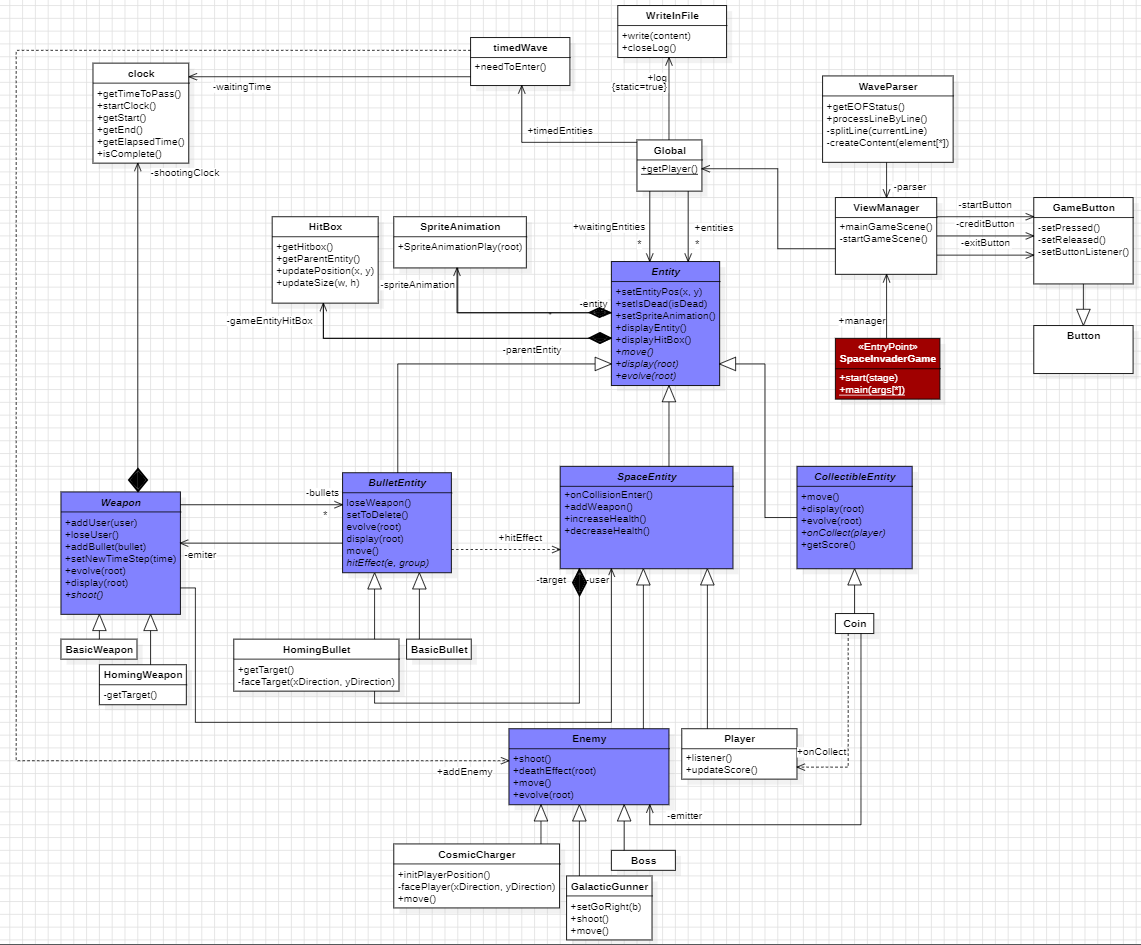
\includegraphics[width=1\textwidth]{images/diagramme.png}
\newline \newline \newline \newline \newline \newline \newline \newline

\subsection{Interfaces}

Lors du lancement du programme dans l'IDE, une première fenêtre s'affiche à l'écran représentant le menu du jeu, composée de plusieurs éléments tels que le logo du jeu, ainsi que les 3 boutons principaux : le bouton \textbf{START}, \textbf{QUIT} et \textbf{COMMANDS} (qui montre comment jouer). En cliquant sur le bouton \textbf{START}, ou en appuyant sur \textbf{ESPACE} ou \textbf{ENTRÉE}, la fenêtre du jeu principal s'affiche. La scène principale du jeu montre un vaisseau en bas de l'écran représentant le joueur, et en face, nous avons les ennemis. Nous avons également la barre de vie du joueur, ainsi qu'un bouton pause. Enfin, nous avons deux autres affichages : le score en haut à droite de l'écran, ainsi que le nombre de points gagnés par le joueur à chaque ennemi tué ou pièce récupérée. Chaque fois que l'on élimine tous les ennemis d'une vague, une nouvelle vague prend sa place. Après quelques vagues, le boss apparaît qu'il faudra battre, avant de voir s'afficher à l'écran l'écriture "\textbf{YOU WIN}" avec le score final ainsi que le plus haut score de toutes les parties jouées.

\subsection{Aspects spécifiques}

Galactic Shooter est un jeu complet, et à donc des algorithmes et des mécaniques complexes et sophistiquées, voici certains algorithmes importants : 
\begin{itemize}
    \item[$\bullet$] Les mouvements des \textbf{BulletEntity} utilisent des algorithmes de trigonmétrie afin d'ajuster continuellement sa direction vers sa cible, ces calculs sont essentiels pour modifier en temps réel l'orientation de l'image du projectile.\newline
    
    \item[$\bullet$] Un algorithme permettant de retranscrire un fichier texte en vagues d'ennemis a été créé (\textbf{WaveParser.java} et \textbf{WaveData.txt} permettant ainsi une grande facilité de création de vagues, sans avoir besoin de modifier le code source du jeu.\newline

    \item[$\bullet$] Une \textbf{HitBox} a été entièrement développé à l'aide de l'objet \textbf{Rectangle} de JavaFX, permettant à chaque entité du jeu d'avoir une véritable boîte de collision et donc d'être intersectable avec les autres entités. Les Rectangles sont ainsi ajouté dans le \textbf{Group root} du jeu, et c'est depuis cet élément que nous traitons les collision.\newline

    \item[$\bullet$] Un algorithme complexe de détection de collisions (\textbf{onCollisionEnter}) a été réalisé afin de détecter les nouvelles collisions entre chaque élément du jeu, et traitant ces collisions en fonction de la classe des objets intragissant entre eux.\newline \newline \newline \newline \newline \newline \newline
    
\end{itemize} 


%----------------------------------------------------------------------
\section{Regard critique}

Dans le jeu Galactic Shooter, nous avons utilisé les concepts fondamentaux de la programmation orientée objet (POO). L'héritage est utilisé constamment, notamment pour la création de toutes les sous-classes de \textbf{Entity}, mais aussi pour les sous-classes de \textbf{Weapon}. Le polymorphisme a aussi été implémenté, avec les différents types de tirs et mouvements des ennemis et du joueur. L'encapsulation est utilisée pour permettre un accès restreint aux attributs privés et donc l'utilisation d'une interface (\textbf{Setters} et \textbf{Getters}), permettant d'interagir de manière sure avec les différents attributs. Les interfaces n'ont néanmoins pas été utilisées car leurs implémentations n'étaient à nos yeux pas intéressantes dans notre idée du projet, nous avons préféré utiliser seulement des classes abstraites(\textbf{Entity}, \textbf{SpaceEntity}, \textbf{CollectibleEntity}, \textbf{BulletEntity} et \textbf{Weapon}).

Le projet a été très sérieusement abordé et étudié dès le premier TP lié au projet, les idées étaient déjà claires et le groupe lucide sur ses compétences et la direction que le projet devait prendre. Nous annoncions à chaque rendez-vous les prochaines taches que nous devions réaliser, et comment nous y prendrons-nous. Aussi, nous avons utilisé Discord pour communiquer sur nos avancés, nos commits sur git, ou pour s'entraider à développer certains algorithmes.

Nous avons constamment travaillait sur le jeu Galactic Shooter depuis le début du projet, et plus nous travaillions, plus les nouvelles idées nous venaient, nous poussant ainsi à travailler encore plus dessus.
Malheureusement l'un de nos membres a été un peu plus en retraite et n'a pas pu fournir autant de travail à ce projet.

Dans ce projet, l'un des membres détenait des connaissances assez avancées en Java, ainsi il a pu nous aider au début du projet pour bien comprendre les fondements du Java et de la POO. Nous nous sommes donc tous entraidés pour être à niveau sur le projet et développer autant l'un que l'autre.

Avec le WaveData.txt et le WaveParser, il est très simple de créer des vagues d'ennemis. Ainsi, il pourrait être possible de facilement renouveler le jeu en y ajoutant de nouveaux ennemis différents. Nous pourrions aussi partir dans l'idée de créer différents niveaux, ou bien aussi de nouvelles armes.

Bien que nous ayons eu directement nos idées et nos méthodes de travail, le professeur encadrant a toujours été à l'écoute de nos interrogations et a su y répondre clairement.

\end{document}
